% Options for packages loaded elsewhere
\PassOptionsToPackage{unicode}{hyperref}
\PassOptionsToPackage{hyphens}{url}
\PassOptionsToPackage{dvipsnames,svgnames,x11names}{xcolor}
%
\documentclass[
]{article}
\usepackage{amsmath,amssymb}
\usepackage{iftex}
\ifPDFTeX
  \usepackage[T1]{fontenc}
  \usepackage[utf8]{inputenc}
  \usepackage{textcomp} % provide euro and other symbols
\else % if luatex or xetex
  \usepackage{unicode-math} % this also loads fontspec
  \defaultfontfeatures{Scale=MatchLowercase}
  \defaultfontfeatures[\rmfamily]{Ligatures=TeX,Scale=1}
\fi
\usepackage{lmodern}
\ifPDFTeX\else
  % xetex/luatex font selection
\fi
% Use upquote if available, for straight quotes in verbatim environments
\IfFileExists{upquote.sty}{\usepackage{upquote}}{}
\IfFileExists{microtype.sty}{% use microtype if available
  \usepackage[]{microtype}
  \UseMicrotypeSet[protrusion]{basicmath} % disable protrusion for tt fonts
}{}
\makeatletter
\@ifundefined{KOMAClassName}{% if non-KOMA class
  \IfFileExists{parskip.sty}{%
    \usepackage{parskip}
  }{% else
    \setlength{\parindent}{0pt}
    \setlength{\parskip}{6pt plus 2pt minus 1pt}}
}{% if KOMA class
  \KOMAoptions{parskip=half}}
\makeatother
\usepackage{xcolor}
\usepackage[margin=1in]{geometry}
\usepackage{color}
\usepackage{fancyvrb}
\newcommand{\VerbBar}{|}
\newcommand{\VERB}{\Verb[commandchars=\\\{\}]}
\DefineVerbatimEnvironment{Highlighting}{Verbatim}{commandchars=\\\{\}}
% Add ',fontsize=\small' for more characters per line
\usepackage{framed}
\definecolor{shadecolor}{RGB}{248,248,248}
\newenvironment{Shaded}{\begin{snugshade}}{\end{snugshade}}
\newcommand{\AlertTok}[1]{\textcolor[rgb]{0.94,0.16,0.16}{#1}}
\newcommand{\AnnotationTok}[1]{\textcolor[rgb]{0.56,0.35,0.01}{\textbf{\textit{#1}}}}
\newcommand{\AttributeTok}[1]{\textcolor[rgb]{0.13,0.29,0.53}{#1}}
\newcommand{\BaseNTok}[1]{\textcolor[rgb]{0.00,0.00,0.81}{#1}}
\newcommand{\BuiltInTok}[1]{#1}
\newcommand{\CharTok}[1]{\textcolor[rgb]{0.31,0.60,0.02}{#1}}
\newcommand{\CommentTok}[1]{\textcolor[rgb]{0.56,0.35,0.01}{\textit{#1}}}
\newcommand{\CommentVarTok}[1]{\textcolor[rgb]{0.56,0.35,0.01}{\textbf{\textit{#1}}}}
\newcommand{\ConstantTok}[1]{\textcolor[rgb]{0.56,0.35,0.01}{#1}}
\newcommand{\ControlFlowTok}[1]{\textcolor[rgb]{0.13,0.29,0.53}{\textbf{#1}}}
\newcommand{\DataTypeTok}[1]{\textcolor[rgb]{0.13,0.29,0.53}{#1}}
\newcommand{\DecValTok}[1]{\textcolor[rgb]{0.00,0.00,0.81}{#1}}
\newcommand{\DocumentationTok}[1]{\textcolor[rgb]{0.56,0.35,0.01}{\textbf{\textit{#1}}}}
\newcommand{\ErrorTok}[1]{\textcolor[rgb]{0.64,0.00,0.00}{\textbf{#1}}}
\newcommand{\ExtensionTok}[1]{#1}
\newcommand{\FloatTok}[1]{\textcolor[rgb]{0.00,0.00,0.81}{#1}}
\newcommand{\FunctionTok}[1]{\textcolor[rgb]{0.13,0.29,0.53}{\textbf{#1}}}
\newcommand{\ImportTok}[1]{#1}
\newcommand{\InformationTok}[1]{\textcolor[rgb]{0.56,0.35,0.01}{\textbf{\textit{#1}}}}
\newcommand{\KeywordTok}[1]{\textcolor[rgb]{0.13,0.29,0.53}{\textbf{#1}}}
\newcommand{\NormalTok}[1]{#1}
\newcommand{\OperatorTok}[1]{\textcolor[rgb]{0.81,0.36,0.00}{\textbf{#1}}}
\newcommand{\OtherTok}[1]{\textcolor[rgb]{0.56,0.35,0.01}{#1}}
\newcommand{\PreprocessorTok}[1]{\textcolor[rgb]{0.56,0.35,0.01}{\textit{#1}}}
\newcommand{\RegionMarkerTok}[1]{#1}
\newcommand{\SpecialCharTok}[1]{\textcolor[rgb]{0.81,0.36,0.00}{\textbf{#1}}}
\newcommand{\SpecialStringTok}[1]{\textcolor[rgb]{0.31,0.60,0.02}{#1}}
\newcommand{\StringTok}[1]{\textcolor[rgb]{0.31,0.60,0.02}{#1}}
\newcommand{\VariableTok}[1]{\textcolor[rgb]{0.00,0.00,0.00}{#1}}
\newcommand{\VerbatimStringTok}[1]{\textcolor[rgb]{0.31,0.60,0.02}{#1}}
\newcommand{\WarningTok}[1]{\textcolor[rgb]{0.56,0.35,0.01}{\textbf{\textit{#1}}}}
\usepackage{graphicx}
\makeatletter
\def\maxwidth{\ifdim\Gin@nat@width>\linewidth\linewidth\else\Gin@nat@width\fi}
\def\maxheight{\ifdim\Gin@nat@height>\textheight\textheight\else\Gin@nat@height\fi}
\makeatother
% Scale images if necessary, so that they will not overflow the page
% margins by default, and it is still possible to overwrite the defaults
% using explicit options in \includegraphics[width, height, ...]{}
\setkeys{Gin}{width=\maxwidth,height=\maxheight,keepaspectratio}
% Set default figure placement to htbp
\makeatletter
\def\fps@figure{htbp}
\makeatother
\setlength{\emergencystretch}{3em} % prevent overfull lines
\providecommand{\tightlist}{%
  \setlength{\itemsep}{0pt}\setlength{\parskip}{0pt}}
\setcounter{secnumdepth}{-\maxdimen} % remove section numbering
\usepackage{booktabs}
\usepackage{caption}
\usepackage{longtable}
\usepackage{colortbl}
\usepackage{array}
\usepackage{anyfontsize}
\usepackage{multirow}
\ifLuaTeX
  \usepackage{selnolig}  % disable illegal ligatures
\fi
\IfFileExists{bookmark.sty}{\usepackage{bookmark}}{\usepackage{hyperref}}
\IfFileExists{xurl.sty}{\usepackage{xurl}}{} % add URL line breaks if available
\urlstyle{same}
\hypersetup{
  pdftitle={STAT 442/842, CM 762 W25 Assignment 2},
  colorlinks=true,
  linkcolor={Maroon},
  filecolor={Maroon},
  citecolor={Blue},
  urlcolor={blue},
  pdfcreator={LaTeX via pandoc}}

\title{STAT 442/842, CM 762 W25 Assignment 2}
\usepackage{etoolbox}
\makeatletter
\providecommand{\subtitle}[1]{% add subtitle to \maketitle
  \apptocmd{\@title}{\par {\large #1 \par}}{}{}
}
\makeatother
\subtitle{DUE: Monday February 17 by 11:59pm EST}
\author{}
\date{\vspace{-2.5em}}

\begin{document}
\maketitle

\subsection{NOTES}\label{notes}

This assignment has 4 programming questions for everyone, and 1
programming question for grad students.

Your assignment must be submitted by the due date listed at the top of
this document, and it must be submitted electronically in .pdf format
via Crowdmark.

This means that your responses for different question parts should begin
on separate pages of your .pdf file. Note that your .pdf solution file
must have been generated by R Markdown. Additionally:

Organization and comprehensibility is part of a full solution.
Consequently, points will be deducted for solutions that are not
organized and incomprehensible. Furthermore, if you submit your
assignment to Crowdmark, but you do so incorrectly in any way (e.g., you
upload your Question 2 solution in the Question 1 box), you will receive
a 5\% deduction (i.e., 5\% of the assignment's point total will be
deducted from your point total).

There are 44 marks for Stat 442 students, and 54 marks for Stat 842
students.

\newpage

This dataset is from an ongoing chess analysis project with Ariel
Sheynzon called ``Queens and False Hydras''. In the dataset each line
represents a board position that happened in a game between two highly
rated players on Lichess.org.

Each board setup has been evaluated by a chess engine (specialist AI)
called Fairy Stockfish, and the evaluation recorded in centipawns of
white player advantage. For example, if the board setup was evaluated to
be 345, that would mean that the white (first) player currently had a
3.45 pawn advantage.

From each position, a target piece was then removed and the board setup
re-evaluated. The difference in the evaluations is the estimated
``removal value'', or \texttt{remove\_value} of the piece. For example
if a k\texttt{N}ight was removed from the \texttt{f3} square on the
board, the evaluation changes by 536 centipawns, implying that the
knight is ``worth'' 5.36 pawns in that situation.

\texttt{loc\_removed} is the location of the piece being removed, in
algebraic notation. This has been split in the prep code below into
\texttt{rank\_removed} (y) and \texttt{file\_removed} (x).

\texttt{target\_piece} indicates which piece was removed (side ignored),
among k\texttt{N}ight, \texttt{B}ishop, \texttt{R}ook, or
\texttt{Q}ueen.

You have the full dataset in
\texttt{Chess\ evals\ 1\ piece\ removed\ 2024-12-23.csv}, but you will
only need a few of the variables for this assignment.

\emph{Lore note: A false hydra is a Dungeons and Dragons creature that
can kill without leaving a trace, similarly, we have removed a piece
from the board without leaving a trace, that is, by not moving another
piece into it.}

\begin{Shaded}
\begin{Highlighting}[]
\FunctionTok{library}\NormalTok{(ggplot2)}
\FunctionTok{library}\NormalTok{(ggridges)}
\FunctionTok{library}\NormalTok{(viridis)}
\FunctionTok{library}\NormalTok{(viridisLite)}
\FunctionTok{library}\NormalTok{(hrbrthemes)}
\NormalTok{extrafont}\SpecialCharTok{::}\FunctionTok{font\_import}\NormalTok{(}\AttributeTok{prompt =} \ConstantTok{FALSE}\NormalTok{)}
\NormalTok{extrafont}\SpecialCharTok{::}\FunctionTok{loadfonts}\NormalTok{(}\AttributeTok{device =} \StringTok{"pdf"}\NormalTok{)}
\NormalTok{tinytex}\SpecialCharTok{::}\FunctionTok{tlmgr\_install}\NormalTok{(}\StringTok{"anyfontsize"}\NormalTok{)}
\end{Highlighting}
\end{Shaded}

Q0) (0 marks) Run the following code to prepare the data. You may need
to \texttt{install.packages("stringr")} first. You should get a simple
table of six rows, and bimodal histogram.

\begin{Shaded}
\begin{Highlighting}[]
\FunctionTok{library}\NormalTok{(stringr)}

\NormalTok{dat\_chess }\OtherTok{=} \FunctionTok{read.csv}\NormalTok{(}\StringTok{"Chess evals 1 piece removed 2024{-}12{-}23.csv"}\NormalTok{)}
\NormalTok{dat\_chess }\OtherTok{=}\NormalTok{ dat\_chess[,}\FunctionTok{c}\NormalTok{(}\StringTok{"target\_piece"}\NormalTok{, }\StringTok{"loc\_removed"}\NormalTok{, }\StringTok{"remove\_value"}\NormalTok{)]}
\NormalTok{dat\_chess }\OtherTok{=} \FunctionTok{subset}\NormalTok{(dat\_chess, }\SpecialCharTok{!}\FunctionTok{is.na}\NormalTok{(remove\_value))}
\NormalTok{dat\_chess }\OtherTok{=} \FunctionTok{subset}\NormalTok{(dat\_chess, remove\_value }\SpecialCharTok{\textless{}} \DecValTok{2000} \SpecialCharTok{\&}\NormalTok{ remove\_value }\SpecialCharTok{\textgreater{}} \DecValTok{0}\NormalTok{)}

\NormalTok{dat\_chess}\SpecialCharTok{$}\NormalTok{remove\_value }\OtherTok{=} \FunctionTok{abs}\NormalTok{(dat\_chess}\SpecialCharTok{$}\NormalTok{remove\_value)}
\NormalTok{dat\_chess}\SpecialCharTok{$}\NormalTok{target\_piece }\OtherTok{=} \FunctionTok{toupper}\NormalTok{(dat\_chess}\SpecialCharTok{$}\NormalTok{target\_piece)}


\NormalTok{dat\_chess}\SpecialCharTok{$}\NormalTok{file\_removed }\OtherTok{=} \ConstantTok{NA}

\NormalTok{dat\_chess}\SpecialCharTok{$}\NormalTok{rank\_removed }\OtherTok{=} 
  \FunctionTok{as.numeric}\NormalTok{(}\FunctionTok{str\_sub}\NormalTok{(dat\_chess}\SpecialCharTok{$}\NormalTok{loc\_removed, }\DecValTok{2}\NormalTok{,}\DecValTok{2}\NormalTok{))}

\ControlFlowTok{for}\NormalTok{(k }\ControlFlowTok{in} \DecValTok{1}\SpecialCharTok{:}\FunctionTok{nrow}\NormalTok{(dat\_chess))}
\NormalTok{\{}
\NormalTok{  dat\_chess}\SpecialCharTok{$}\NormalTok{file\_removed[k] }\OtherTok{=} 
    \FunctionTok{which}\NormalTok{(letters }\SpecialCharTok{==} \FunctionTok{str\_sub}\NormalTok{(dat\_chess}\SpecialCharTok{$}\NormalTok{loc\_removed[k], }\DecValTok{1}\NormalTok{, }\DecValTok{1}\NormalTok{))}
\NormalTok{\}}


\CommentTok{\# take a random sample of }
\NormalTok{sample\_idx }\OtherTok{=} \FunctionTok{which}\NormalTok{(}\FunctionTok{row.names}\NormalTok{(dat\_chess) }\SpecialCharTok{\%in\%} \FunctionTok{c}\NormalTok{(}\DecValTok{26842}\NormalTok{, }\DecValTok{31374}\NormalTok{, }\DecValTok{19103}\NormalTok{, }\DecValTok{778}\NormalTok{, }\DecValTok{27433}\NormalTok{, }\DecValTok{17317}\NormalTok{))}
\NormalTok{dat\_chess[sample\_idx, ]}
\end{Highlighting}
\end{Shaded}

\begin{verbatim}
##       target_piece loc_removed remove_value file_removed rank_removed
## 778              R          f6          834            6            6
## 17317            Q          d1         1307            4            1
## 19103            N          c3          527            3            3
## 26842            N          f3          536            6            3
## 27433            N          f3          560            6            3
## 31374            B          c4          544            3            4
\end{verbatim}

\begin{Shaded}
\begin{Highlighting}[]
\FunctionTok{hist}\NormalTok{(dat\_chess}\SpecialCharTok{$}\NormalTok{remove\_value)}
\end{Highlighting}
\end{Shaded}

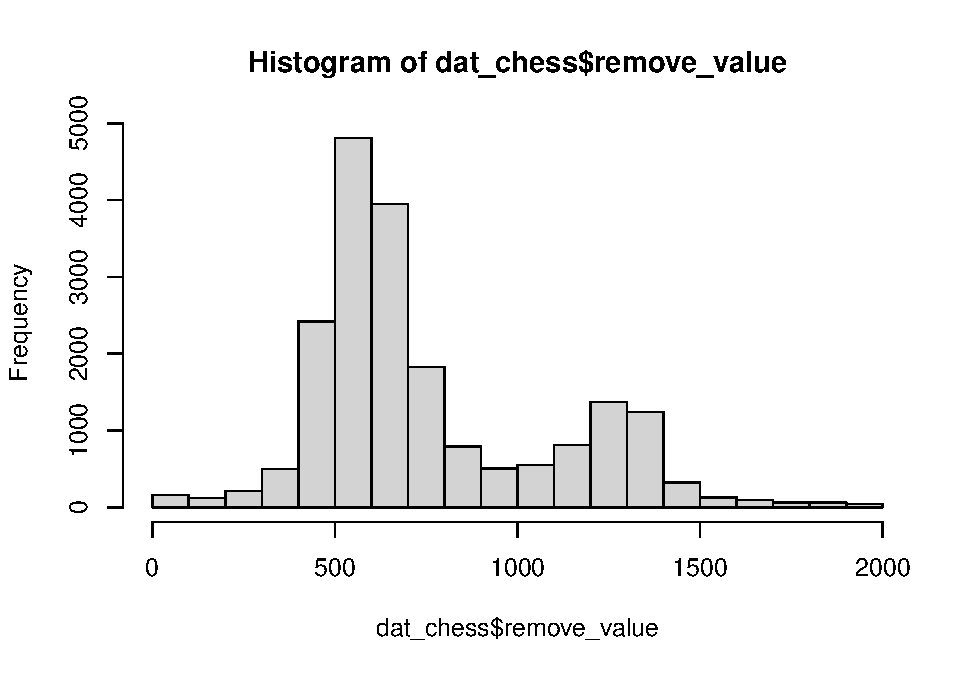
\includegraphics{STAT842_Assignment2_files/figure-latex/unnamed-chunk-2-1.pdf}

\newpage

Q1) Grammar of Tables (12 marks) Make a \texttt{gt} table of the 20 rows
in \texttt{dat\_chess\_q1} in which\ldots{}

\begin{itemize}
\tightlist
\item
  There is a title that says ``Queens and False Hydras''
\item
  There is a subtitle that says ``Value of pieces when removed from the
  chess board''
\item
  The rows are organized from highest to lowest \texttt{remove\_value}
\item
  The \texttt{remove\_value} column is background colour coded so that
  the greatest value is \texttt{\#8888FF} and the least value is
  \texttt{\#22CCFF}.
\item
  The \texttt{target\_piece} column is colour coded so that each of
  \texttt{R}, \texttt{Q}, \texttt{N}, and \texttt{B} has a distinct
  background colour, such that the text is readable.
\item
  The font is the Roboto Google Font
\end{itemize}

Show your code and the resulting table

( You may find this presentation useful:
\url{https://themockup.blog/static/slides/intro-tables-urban.html} )

\begin{Shaded}
\begin{Highlighting}[]
\FunctionTok{library}\NormalTok{(hrbrthemes)}
\FunctionTok{import\_roboto\_condensed}\NormalTok{()}
\FunctionTok{library}\NormalTok{(dplyr)}
\FunctionTok{library}\NormalTok{(gt)}

\NormalTok{q1\_idx }\OtherTok{=} \FunctionTok{seq}\NormalTok{(}\AttributeTok{from=}\DecValTok{1}\NormalTok{, }\AttributeTok{to=}\DecValTok{19001}\NormalTok{, }\AttributeTok{by=}\DecValTok{1000}\NormalTok{) }\CommentTok{\#1, 1001, 2001, 3001, ... , 19001}
\NormalTok{dat\_chess\_q1 }\OtherTok{=}\NormalTok{ dat\_chess[q1\_idx, ]}

\NormalTok{dat\_chess\_q1 }\SpecialCharTok{\%\textgreater{}\%}
    \FunctionTok{arrange}\NormalTok{(}
    \FunctionTok{desc}\NormalTok{(dat\_chess\_q1}\SpecialCharTok{$}\NormalTok{remove\_value)}
\NormalTok{  ) }\SpecialCharTok{\%\textgreater{}\%}
  \FunctionTok{gt}\NormalTok{() }\SpecialCharTok{\%\textgreater{}\%}
  \FunctionTok{tab\_header}\NormalTok{(}
    \AttributeTok{title =} \StringTok{"Queens and False Hydras"}\NormalTok{,}
    \AttributeTok{subtitle =} \StringTok{"Value of pieces when removed from the chess board"}
\NormalTok{  ) }\SpecialCharTok{\%\textgreater{}\%}
  \FunctionTok{data\_color}\NormalTok{(}
    \AttributeTok{columns =} \FunctionTok{vars}\NormalTok{(remove\_value),}
    \AttributeTok{colors =}\NormalTok{ scales}\SpecialCharTok{::}\FunctionTok{col\_numeric}\NormalTok{(}
      \AttributeTok{palette =} \FunctionTok{c}\NormalTok{(}\StringTok{"\#22CCFF"}\NormalTok{, }\StringTok{"\#8888FF"}\NormalTok{),}
      \AttributeTok{domain =} \ConstantTok{NULL}
\NormalTok{    )}
\NormalTok{  ) }\SpecialCharTok{\%\textgreater{}\%}
  \FunctionTok{data\_color}\NormalTok{(}
    \AttributeTok{columns =} \FunctionTok{vars}\NormalTok{(target\_piece),}
    \AttributeTok{colors =}\NormalTok{ scales}\SpecialCharTok{::}\FunctionTok{col\_factor}\NormalTok{(}
      \AttributeTok{palette =} \FunctionTok{c}\NormalTok{(}\StringTok{"\#FF0000"}\NormalTok{, }\StringTok{"\#00FF00"}\NormalTok{, }\StringTok{"\#0000FF"}\NormalTok{, }\StringTok{"\#FF00FF"}\NormalTok{),}
      \AttributeTok{domain =} \FunctionTok{c}\NormalTok{(}\StringTok{"R"}\NormalTok{, }\StringTok{"Q"}\NormalTok{, }\StringTok{"N"}\NormalTok{, }\StringTok{"B"}\NormalTok{)}
\NormalTok{    )}
\NormalTok{  ) }\SpecialCharTok{\%\textgreater{}\%}
  \FunctionTok{tab\_style}\NormalTok{(}
    \AttributeTok{style =} \FunctionTok{list}\NormalTok{(}
      \FunctionTok{cell\_text}\NormalTok{(}
        \AttributeTok{font =} \StringTok{"Roboto"}
\NormalTok{      )}
\NormalTok{    ),}
    \AttributeTok{locations =} \FunctionTok{cells\_body}\NormalTok{(}
\NormalTok{    )}
\NormalTok{  )}
\end{Highlighting}
\end{Shaded}

\begin{table}[!t]
\caption*{
{\large Queens and False Hydras} \\ 
{\small Value of pieces when removed from the chess board}
} 
\fontsize{12.0pt}{14.4pt}\selectfont
\begin{tabular*}{\linewidth}{@{\extracolsep{\fill}}llrrr}
\toprule
target\_piece & loc\_removed & remove\_value & file\_removed & rank\_removed \\ 
\midrule\addlinespace[2.5pt]
{\cellcolor[HTML]{0000FF}{\textcolor[HTML]{FFFFFF}{Q}}} & {d1} & {\cellcolor[HTML]{8888FF}{\textcolor[HTML]{FFFFFF}{1322}}} & {4} & {1} \\ 
{\cellcolor[HTML]{0000FF}{\textcolor[HTML]{FFFFFF}{Q}}} & {d1} & {\cellcolor[HTML]{8889FF}{\textcolor[HTML]{FFFFFF}{1316}}} & {4} & {1} \\ 
{\cellcolor[HTML]{0000FF}{\textcolor[HTML]{FFFFFF}{Q}}} & {a4} & {\cellcolor[HTML]{858DFF}{\textcolor[HTML]{FFFFFF}{1263}}} & {1} & {4} \\ 
{\cellcolor[HTML]{0000FF}{\textcolor[HTML]{FFFFFF}{Q}}} & {d1} & {\cellcolor[HTML]{7E96FF}{\textcolor[HTML]{FFFFFF}{1154}}} & {4} & {1} \\ 
{\cellcolor[HTML]{0000FF}{\textcolor[HTML]{FFFFFF}{Q}}} & {c2} & {\cellcolor[HTML]{5DB5FF}{\textcolor[HTML]{000000}{769}}} & {3} & {2} \\ 
{\cellcolor[HTML]{FF00FF}{\textcolor[HTML]{FFFFFF}{R}}} & {a1} & {\cellcolor[HTML]{54BBFF}{\textcolor[HTML]{000000}{691}}} & {1} & {1} \\ 
{\cellcolor[HTML]{FF00FF}{\textcolor[HTML]{FFFFFF}{R}}} & {a1} & {\cellcolor[HTML]{51BCFF}{\textcolor[HTML]{000000}{671}}} & {1} & {1} \\ 
{\cellcolor[HTML]{FF00FF}{\textcolor[HTML]{FFFFFF}{R}}} & {a1} & {\cellcolor[HTML]{50BCFF}{\textcolor[HTML]{000000}{668}}} & {1} & {1} \\ 
{\cellcolor[HTML]{FF00FF}{\textcolor[HTML]{FFFFFF}{R}}} & {d1} & {\cellcolor[HTML]{4FBDFF}{\textcolor[HTML]{000000}{661}}} & {4} & {1} \\ 
{\cellcolor[HTML]{FF0000}{\textcolor[HTML]{FFFFFF}{B}}} & {c1} & {\cellcolor[HTML]{4CBFFF}{\textcolor[HTML]{000000}{639}}} & {3} & {1} \\ 
{\cellcolor[HTML]{FF00FF}{\textcolor[HTML]{FFFFFF}{R}}} & {a1} & {\cellcolor[HTML]{4AC0FF}{\textcolor[HTML]{000000}{626}}} & {1} & {1} \\ 
{\cellcolor[HTML]{00FF00}{\textcolor[HTML]{000000}{N}}} & {c3} & {\cellcolor[HTML]{44C2FF}{\textcolor[HTML]{000000}{594}}} & {3} & {3} \\ 
{\cellcolor[HTML]{00FF00}{\textcolor[HTML]{000000}{N}}} & {c3} & {\cellcolor[HTML]{3DC5FF}{\textcolor[HTML]{000000}{556}}} & {3} & {3} \\ 
{\cellcolor[HTML]{FF0000}{\textcolor[HTML]{FFFFFF}{B}}} & {f4} & {\cellcolor[HTML]{3AC6FF}{\textcolor[HTML]{000000}{544}}} & {6} & {4} \\ 
{\cellcolor[HTML]{00FF00}{\textcolor[HTML]{000000}{N}}} & {c3} & {\cellcolor[HTML]{36C7FF}{\textcolor[HTML]{000000}{527}}} & {3} & {3} \\ 
{\cellcolor[HTML]{00FF00}{\textcolor[HTML]{000000}{N}}} & {b1} & {\cellcolor[HTML]{35C8FF}{\textcolor[HTML]{000000}{520}}} & {2} & {1} \\ 
{\cellcolor[HTML]{FF00FF}{\textcolor[HTML]{FFFFFF}{R}}} & {d1} & {\cellcolor[HTML]{2CCAFF}{\textcolor[HTML]{000000}{488}}} & {4} & {1} \\ 
{\cellcolor[HTML]{00FF00}{\textcolor[HTML]{000000}{N}}} & {b1} & {\cellcolor[HTML]{2ACAFF}{\textcolor[HTML]{000000}{483}}} & {2} & {1} \\ 
{\cellcolor[HTML]{FF0000}{\textcolor[HTML]{FFFFFF}{B}}} & {c4} & {\cellcolor[HTML]{22CCFF}{\textcolor[HTML]{000000}{462}}} & {3} & {4} \\ 
{\cellcolor[HTML]{FF0000}{\textcolor[HTML]{FFFFFF}{B}}} & {c1} & {\cellcolor[HTML]{22CCFF}{\textcolor[HTML]{000000}{461}}} & {3} & {1} \\ 
\bottomrule
\end{tabular*}
\end{table}

\newpage

Q2) (12 marks) Ridgeline plot.

Draw a ridgeline plot using the \texttt{geom\_density\_ridges()}
geometry in the \texttt{ggridges} package and \texttt{dat\_chess} such
that\ldots{}

\begin{itemize}
\tightlist
\item
  Each row has a KDE of the distribution of \texttt{remove\_value} for
  one of the four pieces
\item
  Each row is labelled with the NAME of the piece (not just the single
  letter code)
\item
  Rows are \texttt{reorder}ed such that the group with the highest mean
  value is placed on the top.
\item
  Each KDE has a different line colour from the \texttt{viridis}
  palette.
\item
  Each KDE uses the same fill gradient from the \texttt{viridis} colour
  scale.
\item
  Clipping is turned off so the top of the KDE doesn't get cut off.
\item
  \texttt{theme\_ipsum()} is used.
\item
  There is no guide or legend shown.
\end{itemize}

You may find
\url{https://wilkelab.org/ggridges/articles/introduction.html} useful,
especially for the fill gradient.

\begin{Shaded}
\begin{Highlighting}[]
\NormalTok{labels }\OtherTok{=} \FunctionTok{c}\NormalTok{(}\StringTok{"Bishop"}\NormalTok{, }\StringTok{"Knight"}\NormalTok{, }\StringTok{"Queen"}\NormalTok{, }\StringTok{"Rook"}\NormalTok{)}

\NormalTok{dat\_chess\_q2 }\OtherTok{\textless{}{-}}\NormalTok{ dat\_chess }\SpecialCharTok{\%\textgreater{}\%}
  \FunctionTok{group\_by}\NormalTok{(target\_piece)}

\NormalTok{dat\_chess\_q2}\SpecialCharTok{$}\NormalTok{target\_piece }\OtherTok{=} \FunctionTok{factor}\NormalTok{(dat\_chess}\SpecialCharTok{$}\NormalTok{target\_piece, }\AttributeTok{levels =} \FunctionTok{c}\NormalTok{(}\StringTok{"B"}\NormalTok{, }\StringTok{"N"}\NormalTok{, }\StringTok{"Q"}\NormalTok{, }\StringTok{"R"}\NormalTok{), }\AttributeTok{labels =}\NormalTok{ labels)}

\FunctionTok{ggplot}\NormalTok{(dat\_chess\_q2, }\FunctionTok{aes}\NormalTok{(}\AttributeTok{x =}\NormalTok{ remove\_value, }\AttributeTok{y =} \FunctionTok{reorder}\NormalTok{(target\_piece, remove\_value, }\AttributeTok{FUN=}\NormalTok{mean), }\AttributeTok{fill =}\NormalTok{ target\_piece)) }\SpecialCharTok{+}
  \FunctionTok{geom\_density\_ridges}\NormalTok{(}\AttributeTok{alpha=}\FloatTok{0.5}\NormalTok{, }\FunctionTok{aes}\NormalTok{(}\AttributeTok{color =}\NormalTok{ target\_piece), }\AttributeTok{scale =} \FloatTok{0.9}\NormalTok{) }\SpecialCharTok{+}
  \FunctionTok{coord\_cartesian}\NormalTok{(}\AttributeTok{clip =} \StringTok{"off"}\NormalTok{) }\SpecialCharTok{+}
  \FunctionTok{scale\_color\_viridis\_d}\NormalTok{() }\SpecialCharTok{+}
  \FunctionTok{scale\_fill\_viridis\_d}\NormalTok{() }\SpecialCharTok{+}
  \FunctionTok{labs}\NormalTok{(}\AttributeTok{x =} \StringTok{"Remove value"}\NormalTok{, }\AttributeTok{y =} \StringTok{"Target Piece"}\NormalTok{,}
       \AttributeTok{title =} \StringTok{"Ridgeline plot of piece removal values"}\NormalTok{) }\SpecialCharTok{+}
  \FunctionTok{theme\_ipsum}\NormalTok{() }\SpecialCharTok{+}
  \FunctionTok{theme}\NormalTok{(}\AttributeTok{legend.position =} \StringTok{"none"}\NormalTok{)}
\end{Highlighting}
\end{Shaded}

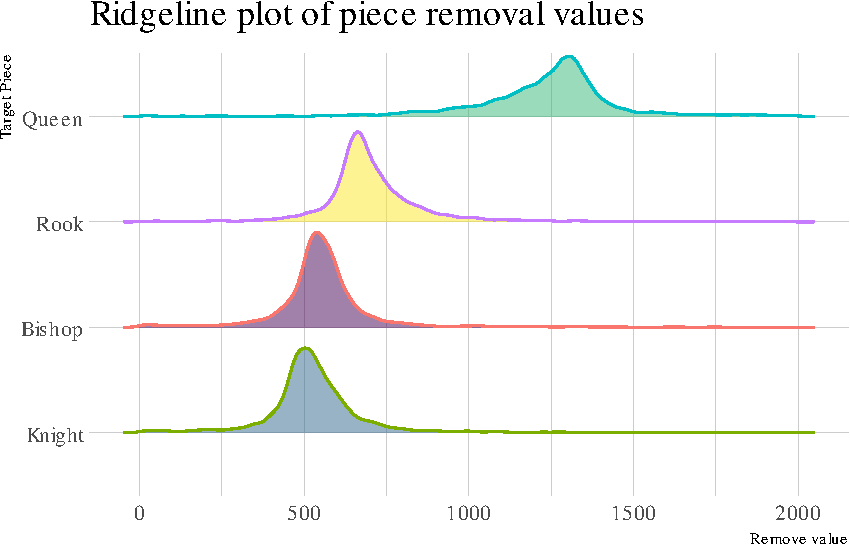
\includegraphics{STAT842_Assignment2_files/figure-latex/unnamed-chunk-4-1.pdf}

\newpage

Q3) (12 marks) Facets and KDEs. ( marks)

Draw a ggplot of \texttt{dat\_chess} using \texttt{geom\_density()} and
\texttt{facet\_wrap()} such that\ldots{}

\begin{itemize}
\tightlist
\item
  Each facet has a KDE of the distribution of \texttt{remove\_value} for
  one of the four pieces.
\item
  Each KDE has a line width of 3.
\item
  The KDE has a line colour of blue, forestgreen, red, or black for
  bishop, knight, queen, and rook respectively.
\item
  The KDE has a fill colour matching the line colour, but at 50\%
  opacity.
\item
  The mean removal value of each piece is written in the top right
  corner (black, bold, any font).
\item
  \texttt{theme\_ipsum()} is used.
\item
  There is no guide or legend shown.
\end{itemize}

For finding the mean removal of each piece, something like
\texttt{by(value,\ piece,\ mean)} or a \texttt{ddply} summarize may be
useful.

\begin{Shaded}
\begin{Highlighting}[]
\FunctionTok{library}\NormalTok{(ggplot2)}
\FunctionTok{library}\NormalTok{(dplyr)}
\FunctionTok{library}\NormalTok{(hrbrthemes)}

\CommentTok{\# Compute mean values using \textasciigrave{}by()\textasciigrave{}, then convert to a data frame}
\NormalTok{mean\_values }\OtherTok{=} \FunctionTok{as.data.frame}\NormalTok{(}\FunctionTok{by}\NormalTok{(dat\_chess}\SpecialCharTok{$}\NormalTok{remove\_value, dat\_chess}\SpecialCharTok{$}\NormalTok{target\_piece, mean))}

\CommentTok{\# Ensure column names are correct}
\FunctionTok{colnames}\NormalTok{(mean\_values) }\OtherTok{\textless{}{-}} \FunctionTok{c}\NormalTok{(}\StringTok{"mean\_val"}\NormalTok{)}
\NormalTok{mean\_values}\SpecialCharTok{$}\NormalTok{target\_piece }\OtherTok{\textless{}{-}} \FunctionTok{rownames}\NormalTok{(mean\_values)  }\CommentTok{\# Convert rownames to a proper column}

\CommentTok{\# Define colors for each piece}
\NormalTok{colors }\OtherTok{=} \FunctionTok{c}\NormalTok{(}\StringTok{"blue"}\NormalTok{, }\StringTok{"forestgreen"}\NormalTok{, }\StringTok{"red"}\NormalTok{, }\StringTok{"black"}\NormalTok{)}

\CommentTok{\#create the plot}
\FunctionTok{ggplot}\NormalTok{(dat\_chess, }\FunctionTok{aes}\NormalTok{(}\AttributeTok{x =}\NormalTok{ remove\_value, }\AttributeTok{fill =}\NormalTok{ target\_piece, }\AttributeTok{color =}\NormalTok{ target\_piece)) }\SpecialCharTok{+}  
  \FunctionTok{geom\_density}\NormalTok{(}\AttributeTok{alpha =} \FloatTok{0.5}\NormalTok{, }\AttributeTok{size =} \DecValTok{3}\NormalTok{) }\SpecialCharTok{+} 
  \FunctionTok{facet\_wrap}\NormalTok{(}\SpecialCharTok{\textasciitilde{}}\NormalTok{target\_piece) }\SpecialCharTok{+}  
  \FunctionTok{geom\_text}\NormalTok{(}\AttributeTok{mapping =} \FunctionTok{aes}\NormalTok{(}\AttributeTok{x =} \ConstantTok{Inf}\NormalTok{, }\AttributeTok{y =} \ConstantTok{Inf}\NormalTok{, }\AttributeTok{label =} \FunctionTok{paste}\NormalTok{(}\StringTok{"Mean:"}\NormalTok{, }\FunctionTok{round}\NormalTok{(mean\_val, }\DecValTok{2}\NormalTok{))),  }
            \AttributeTok{data =}\NormalTok{ mean\_values, }\AttributeTok{hjust =} \DecValTok{1}\NormalTok{, }\AttributeTok{vjust =} \DecValTok{1}\NormalTok{, }\AttributeTok{fontface =} \StringTok{"bold"}\NormalTok{, }\AttributeTok{color =} \StringTok{"black"}\NormalTok{) }\SpecialCharTok{+}
  \FunctionTok{theme\_ipsum}\NormalTok{() }\SpecialCharTok{+}  
  \FunctionTok{theme}\NormalTok{(}\AttributeTok{legend.position =} \StringTok{"none"}\NormalTok{) }\SpecialCharTok{+}  
  \FunctionTok{scale\_color\_manual}\NormalTok{(}\AttributeTok{values =}\NormalTok{ colors) }\SpecialCharTok{+}  
  \FunctionTok{scale\_fill\_manual}\NormalTok{(}\AttributeTok{values =}\NormalTok{ colors)}
\end{Highlighting}
\end{Shaded}

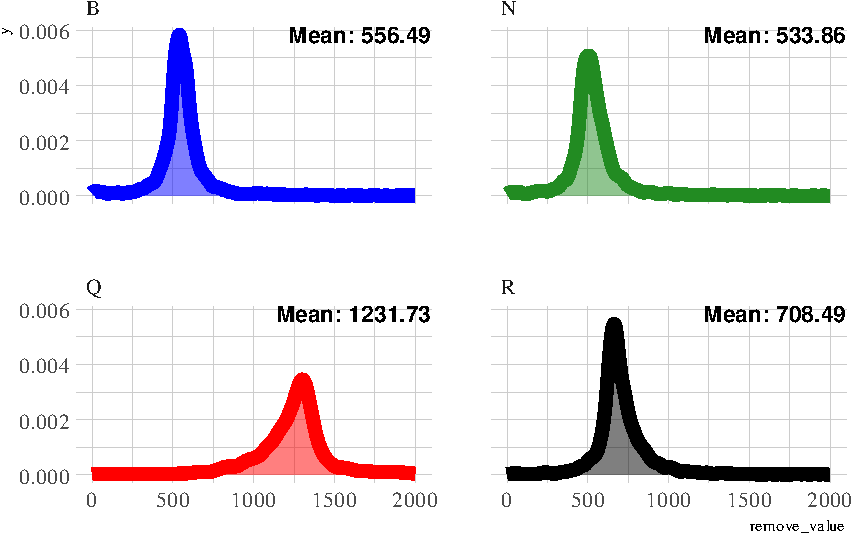
\includegraphics{STAT842_Assignment2_files/figure-latex/unnamed-chunk-5-1.pdf}

\newpage

Q4) (8 marks) Tile plot.

Draw a heatmap of the average removal value (value) of
\texttt{dat\_chess\_q4} using \texttt{geom\_tile()} such that\ldots{}

\begin{itemize}
\tightlist
\item
  The x axis maps to file.
\item
  The y axis maps to rank.
\item
  The fill maps to value.
\item
  The file is labelled with lower case letters a\ldots h.
\item
  The rank is labelled with the numbers 1,2,\ldots,8
\item
  The image \texttt{starting\_position\_algebraic.jpg} (see below) is
  shown underneath the \texttt{geom\_tile}.
\end{itemize}

To add the image, see \texttt{geom\_image()} in
\url{https://www.r-bloggers.com/2024/04/three-ways-to-include-images-in-your-ggplots/}

\begin{Shaded}
\begin{Highlighting}[]
\FunctionTok{library}\NormalTok{(ggimage)}
\FunctionTok{library}\NormalTok{(ggplot2)}
\FunctionTok{library}\NormalTok{(dplyr)}
\FunctionTok{library}\NormalTok{(plyr)}

\NormalTok{dat\_chess\_q4 }\OtherTok{=} \FunctionTok{subset}\NormalTok{(dat\_chess, target\_piece }\SpecialCharTok{==} \StringTok{"N"}\NormalTok{)}

\NormalTok{dat\_chess\_q4 }\OtherTok{=} \FunctionTok{ddply}\NormalTok{(dat\_chess\_q4, }\StringTok{"loc\_removed"}\NormalTok{, summarize,}
                     \AttributeTok{file =}\NormalTok{ file\_removed[}\DecValTok{1}\NormalTok{],}
                     \AttributeTok{rank =}\NormalTok{ rank\_removed[}\DecValTok{1}\NormalTok{],}
                     \AttributeTok{value =} \FunctionTok{mean}\NormalTok{(remove\_value),}
                     \AttributeTok{count =} \FunctionTok{length}\NormalTok{(remove\_value))}

\NormalTok{dat\_chess\_q4}\SpecialCharTok{$}\NormalTok{filename }\OtherTok{=}\NormalTok{ letters[dat\_chess\_q4}\SpecialCharTok{$}\NormalTok{file]}

\NormalTok{plot }\OtherTok{\textless{}{-}} \FunctionTok{ggplot}\NormalTok{(dat\_chess\_q4, }\FunctionTok{aes}\NormalTok{(}\AttributeTok{x =}\NormalTok{ file, }\AttributeTok{y =}\NormalTok{ rank, }\AttributeTok{fill =}\NormalTok{ value)) }\SpecialCharTok{+}
  \FunctionTok{geom\_tile}\NormalTok{() }\SpecialCharTok{+}
  \FunctionTok{scale\_fill\_viridis}\NormalTok{() }\SpecialCharTok{+}
  \FunctionTok{scale\_x\_continuous}\NormalTok{(}\AttributeTok{breaks =} \DecValTok{1}\SpecialCharTok{:}\DecValTok{8}\NormalTok{, }\AttributeTok{labels =}\NormalTok{ letters[}\DecValTok{1}\SpecialCharTok{:}\DecValTok{8}\NormalTok{]) }\SpecialCharTok{+}
  \FunctionTok{scale\_y\_continuous}\NormalTok{(}\AttributeTok{breaks =} \DecValTok{1}\SpecialCharTok{:}\DecValTok{8}\NormalTok{) }\SpecialCharTok{+}
  \FunctionTok{theme\_minimal}\NormalTok{() }\SpecialCharTok{+}
  \FunctionTok{theme}\NormalTok{(}\AttributeTok{legend.position =} \StringTok{"none"}\NormalTok{,}
        \AttributeTok{axis.title =} \FunctionTok{element\_blank}\NormalTok{(),}
        \AttributeTok{panel.grid =} \FunctionTok{element\_blank}\NormalTok{(),}
        \AttributeTok{panel.background =} \FunctionTok{element\_rect}\NormalTok{(}\AttributeTok{fill =} \StringTok{"white"}\NormalTok{))}


\FunctionTok{ggbackground}\NormalTok{(plot, }\StringTok{"starting{-}positon{-}algebraic.jpg"}\NormalTok{) }\SpecialCharTok{+}
  \FunctionTok{geom\_image}\NormalTok{(}\FunctionTok{aes}\NormalTok{(}\AttributeTok{image =} \StringTok{"starting{-}positon{-}algebraic.jpg"}\NormalTok{), }
             \AttributeTok{x =} \FloatTok{0.6}\NormalTok{, }\AttributeTok{y =} \FloatTok{0.6}\NormalTok{, }
             \AttributeTok{xmin =} \DecValTok{2}\NormalTok{, }\AttributeTok{xmax =} \DecValTok{10}\NormalTok{, }\AttributeTok{ymin =} \DecValTok{1}\NormalTok{, }\AttributeTok{ymax =} \DecValTok{8}\NormalTok{) }\SpecialCharTok{+}
  \FunctionTok{coord\_fixed}\NormalTok{(}\AttributeTok{ratio =} \DecValTok{1}\NormalTok{) }
\end{Highlighting}
\end{Shaded}

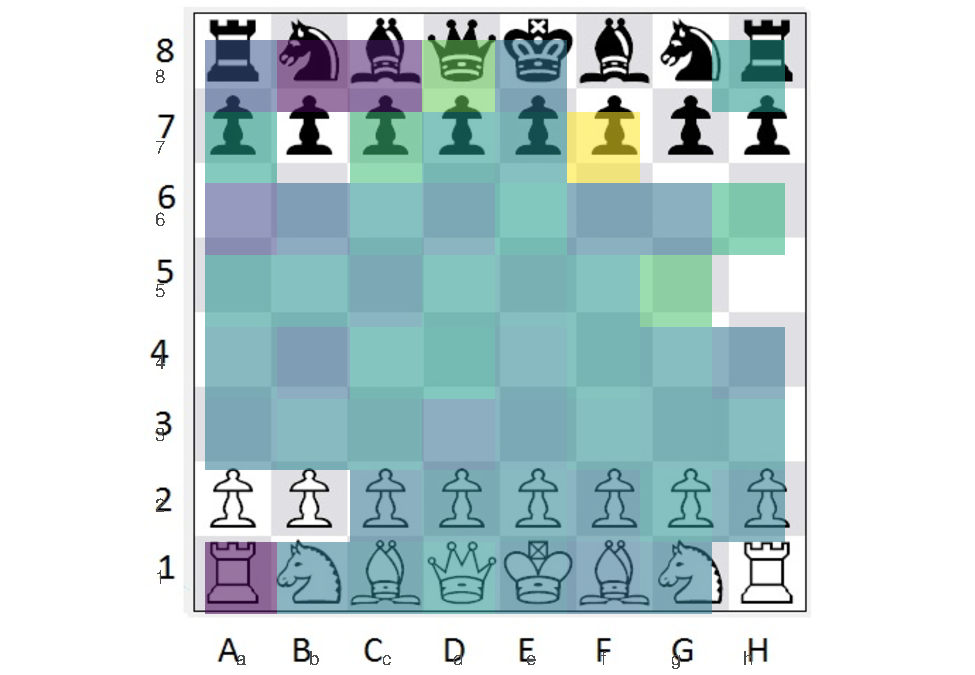
\includegraphics{STAT842_Assignment2_files/figure-latex/unnamed-chunk-6-1.pdf}

\newpage

\textbf{(Stat 842 and CM 762 only. Stat 442 students may attempt this
question, but it will not be marked)}

Q5) (10 marks) Manim histogram.

Using the defaults in the Jan 31 lab, construct a histogram of all the
removal values in Manim using 20 bars.

\begin{itemize}
\tightlist
\item
  Using 20 bars.
\item
  Setting a y-axis tick mark every 500.
\item
  Setting the y-axis from 0 to 5000.
\item
  Setting the background to white.
\item
  Setting a title above the middle of the graph of ``Histogram of Piece
  Values''
\end{itemize}

Hint 1: In the Jupyter notebook, hold shift and right-click in order to
save an image.

Hint 2: In R markdown, you can embed an image with
\texttt{!{[}{]}(filename.png)}

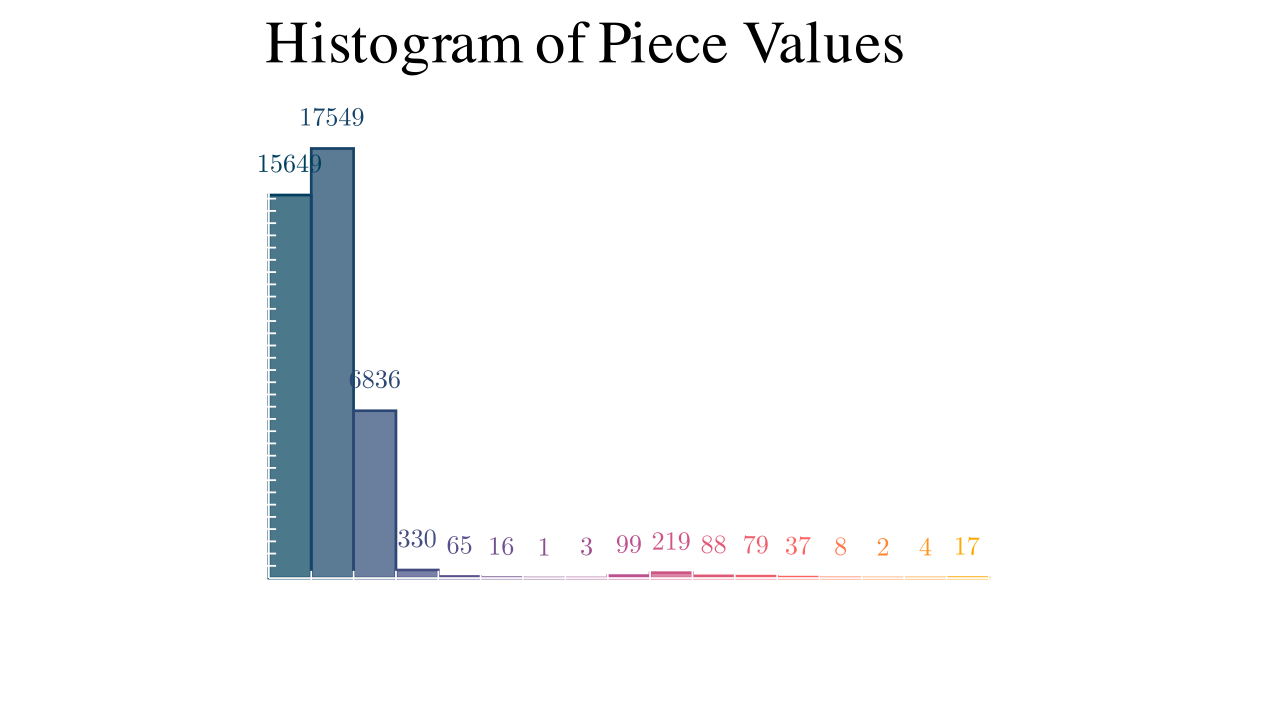
\includegraphics{Histogram_of_Piece_remove.png}

\end{document}
